\documentclass{standalone}
\usepackage[utf8]{inputenc}
\usepackage[T1]{fontenc}
\usepackage{graphicx}
\usepackage{color}
\usepackage{tikz}
\usepackage{pgfplots}
\pgfplotsset{compat=1.11}
\usetikzlibrary{patterns, pgfplots.fillbetween}

% f(x,y) = y
% c(x) = x*(x-1)*(x-2.3)*(x-3.3)+2.3

\begin{document}
  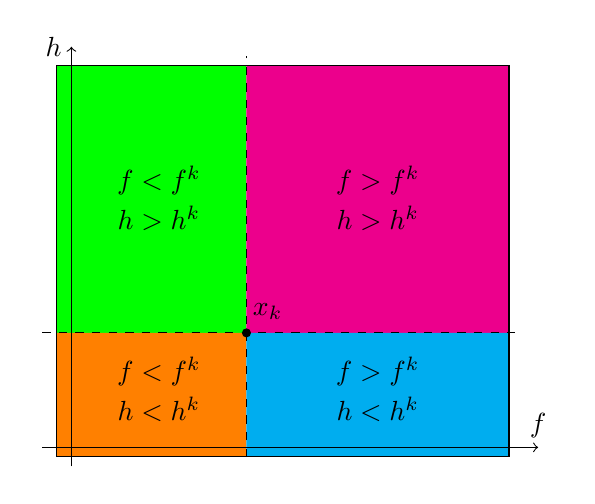
\begin{tikzpicture}
    \def\r{sqrt(2)}
  \begin{axis}[axis lines=none,
      view={0}{90}, mark=none, samples=200, samples y=50,
      xmin=-0.3, xmax=3.4, ymin=-0.3, ymax=4.4,
      domain=-0.2:3]

    \begin{scope}[domain=-0.1:1.2]
      \addplot[name path=A, mark=none, draw=none] (x,4);
      \addplot[name path=B, mark=none, draw=none] (x,1.2);
      \addplot[name path=C, mark=none, draw=none] (x,-0.1);
    \end{scope}
    \begin{scope}[domain=1.2:3]
      \addplot[name path=D, mark=none, draw=none] (x,4);
      \addplot[name path=E, mark=none, draw=none] (x,1.2);
      \addplot[name path=F, mark=none, draw=none] (x,-0.1);
    \end{scope}

    \addplot[green]   fill between[of=A and B];
    \addplot[orange]  fill between[of=B and C];
    \addplot[magenta] fill between[of=D and E];
    \addplot[cyan]    fill between[of=E and F];

    \draw[dashed] (-0.2,1.2) -- (3.1,1.2);
    \draw[dashed] (1.2,-0.1) -- (1.2,4.1);
    \draw[->] (-0.2,0) -- (3.2,0) node[above] {$f$};
    \draw[->] (0,-0.2) -- (0,4.2) node[left] {$h$};
    \draw (-0.1,-0.1) rectangle (3,4);
    \draw[fill,circle] (1.2,1.2) node[above right] {$x_k$} circle (0.05cm);

    \node at (0.6,2.8) {$f < f^k$};
    \node at (0.6,2.4) {$h > h^k$};
    \node at (0.6,0.8) {$f < f^k$};
    \node at (0.6,0.4) {$h < h^k$};
    \node at (2.1,2.8) {$f > f^k$};
    \node at (2.1,2.4) {$h > h^k$};
    \node at (2.1,0.8) {$f > f^k$};
    \node at (2.1,0.4) {$h < h^k$};
  \end{axis}
  \end{tikzpicture}
\end{document}
